% !TeX root = ../main.tex
% -*- coding: utf-8 -*-

\chapter{基于层次注意力网络的函数名推荐}
为了提高代码的易读性和易理解性,本章针对常见的软件重构操作--函数重命名重构进行研究。本章首先阐述了函
数名对软件系统的可维护性的重要性,然后介绍了关于函数重命名的相关研究现状。针对函数内在的层次结构,本
章提出了基于层次注意力网络模型的函数名推荐方法,该方法利用层次注意力网络,学习对函数中的源代码的分布
式表示,并利用该分布式表示预测函数名。在推荐阶段,通过集束搜索生成候选函数名序列,并按序推荐函数名,
从而帮助软件维护人员提高软件系统的可维护性。

\section{研究背景与研究动机}
随着软件系统规模越来越大,软件维护的难度也越来越高。一方面,随着需求的不断增加,软件规模不断增大,导
致软件系统的复杂度越来越高,可维护性降低。另一方面,软件维护通常建立在对软件系统理解的基础上,而合作
的开发模式和人员流动性导致软件维护人员经常需要面对大量陌生的代码,如何快速理解并掌握系统源代码成为维
护人员经常需要面对的问题。

易读性是软件可维护性的重要组成方面,也是评估软件系统质量的关键因素~\cite{buse2008metric}。研究者认
为,在软件维护过程中,最耗费时间和精力成本的是阅读代码的过程~\cite{rugaber2000use}。研究发现,大多数
软件维护人员花费在阅读和理解代码上的时间比真正花费在写代码上的时间更多~\cite{ko2006exploratory}。正
因为此,部分研究者提出在软件维护过程中,需要为阅读和理解代码预留出特定的时间,将代码易读性作为代码检
查的重要指标之一。

为了适应快速迭代的软件需求,当面对大规模软件系统时,软件维护人员通常不需要完全理解和掌握代码的所有细
节,才能对软件系统进行维护。在实践中较为常见的做法是通过阅读函数的标题来理解函数的大致功能,通过多次
跳转快速定位到与当前任务相关的代码位置~\cite{starke2009searching}。只有当通过函数标题无法满足对函数
理解的需求时,才会仔细阅读具体的代码,获得更多的信息。

准确的函数名可以提高代码阅读的速度,从而提高软件维护的效率。在软件维护过程中,维护人员通过快速阅读代
码来理解程序的功能和行为。根据SRP原则~\cite{martin2003agile}(``Single Responsibility
Principle''),每个函数执行一个单独的功能,因此函数通常被认为是程序行为的最小单元
~\cite{host2009debugging}。准确的函数名能够总结函数的功能,因此通过阅读函数名,软件维护人员可以快
速理解函数的整体行为;相反,不准确的函数名通常导致理解和维护软件系统的难度提高
~\cite{arnaoudova2016linguistic},甚至在某些情况下可能导致代码缺陷~\cite{abebe2012can}。

函数重命名是完善性软件维护的重要手段。随着版本的不断更迭,新功能不断被添加,原本合适的函数名也可能变
得不再合适。此时,为了提高程序的易读性,防止由于函数名造成误导,需要进行函数重命名(Rename
Method),在不改变程序行为的前提下,通过更改函数名,提高软件系统的易读性和可维护性。Murphy等人
~\cite{Murphy-Hill:ICSE09}通过对13000位使用Eclipse的Java开发者进行调研,发现函数重命名是最常用的软件
重构类型之一。

尽管函数名对软件系统的易读性和可维护性具有较大的影响,但寻找具有总结能力且易读性强的函数名十分困难
~\cite{allamanis2015suggesting}。寻找好的函数名通常需要在理解函数的基础上,高度抽象整个函数的功能。
近年来,随着自然语言处理领域的不断发展,部分研究者将程序语言作为用来传递指令的一种特殊语言,将代码作
为一种特殊的文本进行学习。例如,Oda等人~\cite{oda2015learning}使用机器翻译技术将Python代码翻译成伪代
码,从而生成易读性更强的代码;Iyer等人~\cite{iyer2016summarizing}设计了一个将代码翻译成文本的神经注
意力模型,将长短期记忆神经网络(LSTM)和注意力机制应用于源代码和自然语言之间的翻译;
Movshovitz-Attias和Cohen~\cite{movshovitz2013natural}使用$n$-gram模型和主题模型从代码中生成评论。

尽管编程语言与自然语言之间存在一定的相似性,但其与自然语言在结构上有很大的区别。虽然自然语言的语法也
存在一定的结构性,但与程序语言相比,自然语言更加序列化和平铺直叙。与自然语言不同,程序语言中蕴含着丰
富的结构信息,直接将代码当做普通文本进行学习,得到的上下文信息不够准确,因此导致模型效果欠佳。

为了充分利用代码中的上下文信息,部分研究者~\cite{allamanis2015suggesting, haiduc2010supporting}通过
程序分析,从源代码中提取出一组与程序语义相关的特征,如Cyclomatic复杂度、变量类型和返回类型等,来表示
代码段。尽管这样的方法可以在一定程度上可以捕获到更精确的代码属性,但该方法依赖于特征工程的有效性,且
人为筛选特征的过程容易遗漏掉更多的语义信息。除此以外,Allamanis等人
~\cite{allamanis2016convolutional}提出使用卷积神经网络来学习代码的结构信息,通过加入注意力网络学习代
码对函数名预测的重要性。虽然卷积神经网络通常被认为适合学习结构特征,但卷积神经网络学到的是位置上的局
部特征,并非代码语义上的局部特征,因此导致其所捕获的上下文信息不够准确。

本文通过程序分析,将函数表示为由代码基本块组成的代码片段,利用代码的原始特征学习代码片段的分布式表示
(Distributed Representation)。与自然语言不同,代码具有明确的控制流结构,将程序行为拆分为多个由基本
块组成的子功能,每个基本块代表一个最小的功能单元;同时,一个代码块由多个词条组成,词条中含有丰富的语
义信息。基于这样的层次结构,本文通过使用层次注意力模型,分别学习代码基本块和词条(token)的重要性,
从而得到函数体的分布式表示并预测函数名。

本章主要有以下贡献:

(1)本章提出了基于层次注意力网络的函数名推荐模型,通过学习函数体的分布式表示,利用序列到序列模型为
给定函数推荐函数名。

(2)本章利用代码的层次结构,将代码表示为由基本块组成的代码片段,使用原始特征学习代码片段的分布式表
示,在代码搜索、克隆代码检测等领域有广泛的应用。

(3)在开源软件系统上的对比实验证明了基于层次注意力网络的函数名推荐模型的准确性,提高了软件维护的效
率。

\section{相关研究工作}
本节首先介绍了代码分布式表示模型,这些模型通过学习对代码的中间表示,将代码片段表示为难以直接解释的向
量。然后介绍了与代码相关的结构化预测模型,最后介绍了关于代码与文本相互转换的模型。

\subsection{分布式表示模型}
在局部表示中,向量中的每个值通常有具体的明确的含义,例如在One-Hot表示模型中,当第$i$维数值为0时,表
示其对应的元素没有现在该样本中。与局部表示不同,分布式表示~\cite{hinton1984distributed}假设所表示
的元素可以在多维实数空间内进行编码,并且可以在该空间内评估两个表示之间的相关性。因此,分布式表示的结
果通常是一种矢量或矩阵,其元素的含义分布在多个维度上。由于具有较好的总结能力,分布式表示经常在自然语
言处理领域中被用来对自然语言中的元素进行编码。例如,Mikolov等人~\cite{mikolov2013efficient}通过学
习自然语言中单词的分布式表示,学到了单词之间的相关性。

\subsection{代码的分布式表示}
由于在机器学习和自然语言处理上的成功运用,近年来,越来越多的研究者使用分布式表示模型表示代码,将代码
元素映射到矢量中。代码表示模型类似于自然语言处理中的文本分类和情感分析系统,使用代码的抽象表示作为输
入,得到关于代码属性的条件概率分布并进行预测。

代码表示模型可用来预测代码片段的属性概率分布,如变量和函数名等。Allamanis等人
~\cite{allamanis2015suggesting}发现变量和函数名的分布式表示可以学到常见的语义属性,使用上下文信息学
习变量和函数的分布式矢量表示,并使用这种表示来预测变量名和函数名的概率分布。Mou等人
~\cite{mou2016convolutional}使用自定义的卷积神经网络来学习代码片段的分布式矢量表示,然他们混合了学生
对各种课程问题的解决方案,通过分类来恢复这些解决方案到问题的映射。Piech等人~\cite{piech2015learning}
和Parisotto等人~\cite{parisotto2017neuro}学习了源代码输入/输出对的分布式表示,并使用这些表示来评估和
审查学生任务。

除此以外,部分研究使用分布式表示来学习上下文信息并生成代码。例如,Maddision等人
~\cite{maddison2014structured}通过对上下文进行分布式表示,按序生成代码。Ling等人
~\cite{ling2016latent}和Allamanis等人~\cite{allamanis2015bimodal}将代码上下文分布式表示与自然语言的
分布式表示相结合来合成代码。



\subsection{代码属性预测}
近年来,越来越多的研究者通过构建关于代码的概率模型,预测代码的属性。Raychev等人
~\cite{raychev2015predicting}将代码表示为变量依赖关系网络,将每个javaScript变量表示为一个节点,并
将其中的变量交互建模为条件随机场(CRF),最后通过联合预测代码片段中所有变量的类型和名称。Allamanis等
人~\cite{allamanis2014learning,allamanis2015suggesting,allamanis2016convolutional}利用代码上下文,使
用分布式表示来预测变量名、函数名和类的名称。


受统计机器翻译启发,Gu等人~\cite{gu2016deep}引入序列到序列的深度神经网络
~\cite{sutskever2014sequence},学习了自然语言查询的中间表示,并用来预测相关的API调用序列。Murali等人
~\cite{murali2017finding}利用主题模型的组合来学习一个循环神经网络,该神经网络为API调用序列建模。该模
型可来检测可能性极小的API调用序列,从而检测Android代码中实际存在的缺陷。

除此以外,Allamanis等人~\cite{allamanis2018learning}还通过学习将代码片段粘贴到现有的代码中,并调整所
使用的变量来预测代码的数据流图。Livshits等人~\cite{livshits2009merlin}通过分布式表示来解决信息流问
题。Allamanis等人~\cite{allamanis2018learning}使用代码上下文中的各种元素来检测特定类型的缺陷,如变量
和操作符误用等。


\subsection{注释和文档生成}
通过学习代码与自然语言文本的关系,可以自动生成代码文档,增加代码可读性。Oda等人
~\cite{oda2015learning}使用机器翻译技术将Python代码翻译成伪代码,从而生成易读性更高的代码;Iyer等
人~\cite{iyer2016summarizing}设计了一个将代码总结为文本的神经注意力模型。Movshovitz等人
~\cite{movshovitz2013natural}构建了一个推荐系统用来在给定源代码片段的情况下协助完成评论,该系统使用
类似主题的图模型来为上下文信息建模。

根据代码生成文本还可以用来自动生成注释。Sridhara等人~\cite{sridhara2010towards}提出了一种使用程序
结构信息为java函数生成摘要注释的方法,该方法的基本思想是从函数中选出重要的语句,然后将其翻译成自然语
言。该方法首先构建函数的数据流程图,然后分析该数据流来识别重要的语句。Wong等人
~\cite{wong2013autocomment}通过问答网站自动生成评论,从问题标题和回答文本中提取代码和描述的映射,
并使用代码克隆检测技术来查找与该映射相近的代码片段,查找出来的代码对通常是由开发人员从项目中复制的代
码,然后识别该代码片段的注释并重新应用于其他项目。然而,虽然这种方法可以应用于数百万个项目,但是其仅
对小部分代码片段有效,但无法为某个项目生成大量注释。

\section{问题描述与研究动机}\label{motivation3}
本文主要解决的是函数命名问题,即为代码片段预测具有语义的标识符。准确的函数名并不是简单描述代码的行
为,而是对代码段语义和功能的总结,因此好的函数名能够提高代码的易读性和易理解性,从而提高软件维护的效
率~\cite{takang1996effects}。

图~\ref{stop}中展示了来自Cassandra的示例代码片段以及本文方法的预测结果。Cassandra是一个开源的分布式
NoSQL数据库系统,其中函数的数量超过一万。当面对如此大规模的软件系统时,几乎一半的软件维护时间被用来
理解代码涵义上~\cite{corbi1989program}。为大型软件系统推荐具有语义的标识符作为函数名,能够减少维护人
员花费在阅读和理解代码上的时间。如图~\ref{stop}所示,本文使用基于层次注意力网络的模型,为示例代码片
段推荐了函数名候选列表,并为列表中的每个函数名分配了一个概率,按照概率由高至低推荐给用户。

虽然函数名重构对于提升软件易读性和可维护性有着重要的作用,但自动生成具有语义的函数名仍然存在以下困
难:

(1)不同于注释或者文档,函数名为由少数子词项(subtoken)组成的标识符,因此函数名推荐需要在非常有限
的空间里总结函数的功能,同时忽略实现细节,这就要求模型具有较强的抽象能力和高层次的总结能力。

(2)不同于自然语言中的文本,程序代码具有高度结构性,通过明确的控制流结构将整体功能拆分成多个子功
能,因此学习并利用代码的结构信息,这就要求模型具有一定的结构学习能力。

(3)虽然函数名在整体上是对函数功能的总结和概括,但由于个人的命名习惯不同,导致很难推荐适用于所有用
户的函数名。

为了解决上述问题,本章提出了基于层次注意力网络的函数名推荐模型,利用代码的层次结构,将函数体拆分为多
个代码基本块,每个代码基本块由多个子词项组成;利用注意力机制分别学习子词项对基本块、基本块对函数体的
重要性,使模型能够识别对函数名预测有益的代码基本块和词项。最后,由于软件系统内部的代码风格通常较为一
致,因此通过使用相同软件系统中的函数命名实例作为训练数据集集,能够为用户推荐符合个性化命名习惯的函数
名。

除此以外,函数命名问题也是一种代码表示问题,即将代码表示为具有语义的矢量,使得具有相似语义的代码片段
能够有相近的表示。本章通过引入层次注意力网络,模拟代码段内部的层次结构,对给定代码片段进行分布式表
示,并学习基于分布式表示的函数名分布的条件概率,从而为给定代码片段预测函数名。除了预测标识符(变量
名、函数名和类名)以外,代码的分布式表示研究在克隆检测~\cite{white2016deep,allamanis2018learning}、
缺陷预测~\cite{murali2017finding}等领域也有广泛的应用。

\begin{figure}
\centering
\subfigure{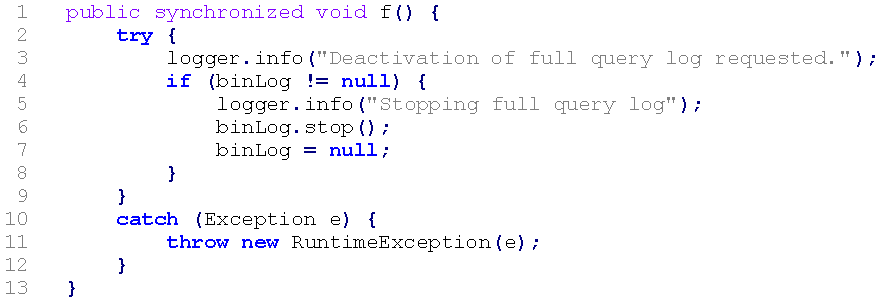
\includegraphics[width=0.82\linewidth]{stop.pdf}}
\hfill
\subfigure{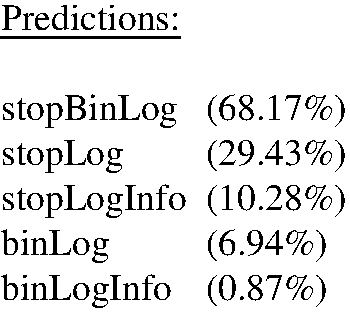
\includegraphics[width=0.17\linewidth]{prediction.pdf}}
\caption{示例代码段以及函数名预测}
\label{stop}
\end{figure}

\section{研究方法}
本章提出了基于层次注意力网络的函数名推荐模型,该模型以编码-解码模型~\cite{Kyunghyun2014Learning}
(Encoder-Decoder)为基本框架,通过输出子词项序列(Subtoken Sequence)来为给定代码片段预测函数名。本
节首先简要阐述编码器-解码器的原理,然后介绍本章的模型架构,接下来依次介绍模型架构的各个组成部分,包
括代码片段的输入表示、编码器、解码器等;最后描述在预测阶段,针对给定的代码段,如何利用训练好的模型使
用集束搜索(Beam Search)生成具有概率的函数名列表。

\subsection{编码-解码模型}
编码-解码模型为常见的一种模型框架,其核心思想是将输入$x$通过编码转化为一个向量$C$,再将向量$C$通过解
码转化为输出$y$。其中用来编码的模型为编码器(Encoder),用来解码的模型为解码器(Decoder)。编码器和
解器均可以为任意的模型,如CNN、RNN、GRU等;输入和输出也可以是任意的形式,如文字、图像等。当$x$和$y$
均为序列时,这样的模型也被称为序列到序列模型(Seq2Seq)。在实际应用中存在很多序列到序列的问题,例如
翻译、问答系统等。

图~\ref{fig:seq2seq}为一个序列到序列模型的例子,其中编码器和解码器均使用循环神经网络(Recurrent Neural
Networks, 简称RNN)。给定输入序列$x=\{x_1,x_2,...,x_m\}$,该模型使用RNN将输入序列$x$编码为一个固定长
度的向量$C$,然后使用RNN将向量$c$解码为输出序列$y=\{y_1,y_2,...,y_n\}$,从而学习关于输出序列$y$在输
入序列$x$上的条件分布。在RNN中,第$t$个时刻的隐藏状态用$h_t$表示,该隐藏状态由前一个隐藏状态
$h_{t-1}$和第$t$个时刻的输入$x_t$共同决定:
\begin{eqnarray}
    h_t = f(h_{t-1},x_t),
\end{eqnarray}
因此,当输入完成时,当前隐藏状态$h_m$中包含了整个输入序列$x$的信息,通常将其作为输入序列$x$的编码
$C$。在解码阶段,同样使用RNN,以$C$作为输入,生成输出序列$y$,不同的是,生成$y_t$的概率还需要考虑已
经生成的输出$y_1,y_2...y_{t-1}$:
\begin{eqnarray}
    p(y_t|y_1,y_2,...,y_{t-1},C) = g(y_{t-1},H_t,C).
\end{eqnarray}
其中第$t$个时刻的隐藏状态$H_t$由前一个时刻的隐藏状态$H_{t-1}$和输出$y_{t-1}$以及输入的编码$C$共同决定:
\begin{eqnarray}
    H_t = f(H_{t-1},y_{t-1},C).
\end{eqnarray}
通过这样的方式,可以在输入序列的长度$m$和输出序列的长度$n$不相等的情况下,构建一个关于输出序列$y$在
输入序列$x$上的条件分布的生成模型$p(y_1,y_2,...,y_n|x_1,x_2,...,x_m)$,然后通过最大似然的方式拟合数
据集。

\begin{figure} [!t]
	\centering
	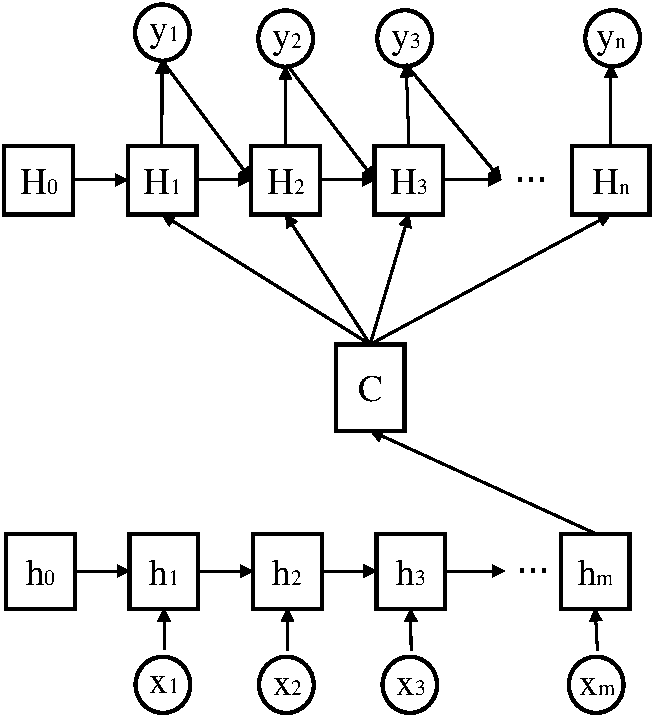
\includegraphics[width=0.95\textwidth]{seq2seq.pdf}
	\caption{RNN编码-解码模型}
	\label{fig:seq2seq}
\end{figure}

本章提出的基于层次注意力网络的函数名推荐模型,与上述模型有相似的架构,均为序列到序列的编码-解码模
型。两者的区别是,本文使用层次注意力网络作为编码器将代码段表示为固定长度的向量,然后使用GRU序列模型
作为解码器,通过学习函数名关于代码段的条件概率分布,输出构成函数名的子词项(Subtoken)序列。

\subsection{函数名推荐模型的基本架构}
本章模型的架构如图~\ref{fig:arch}所示。可以看出,该模型为编码-解码模型
~\cite{Kyunghyun2014Learning}。为了提高模型的抽象和总结能力,本文使用程序分析将函数功能拆分为多个由
代码基本块组成的子功能,不同代码基本块对预测函数名的重要性不同;同时,一个代码块由多个词项组成,不同
的词项的重要性也不同。为了模拟这样的层次结构,在编码阶段引入层次注意力模型
~\cite{yang2016hierarchical}分别学习代码基本块和词条(token)对预测函数名的重要性,通过编码-解码模型
学习函数名在代码片段上的条件分布。

\begin{figure} [!t]
	\centering
	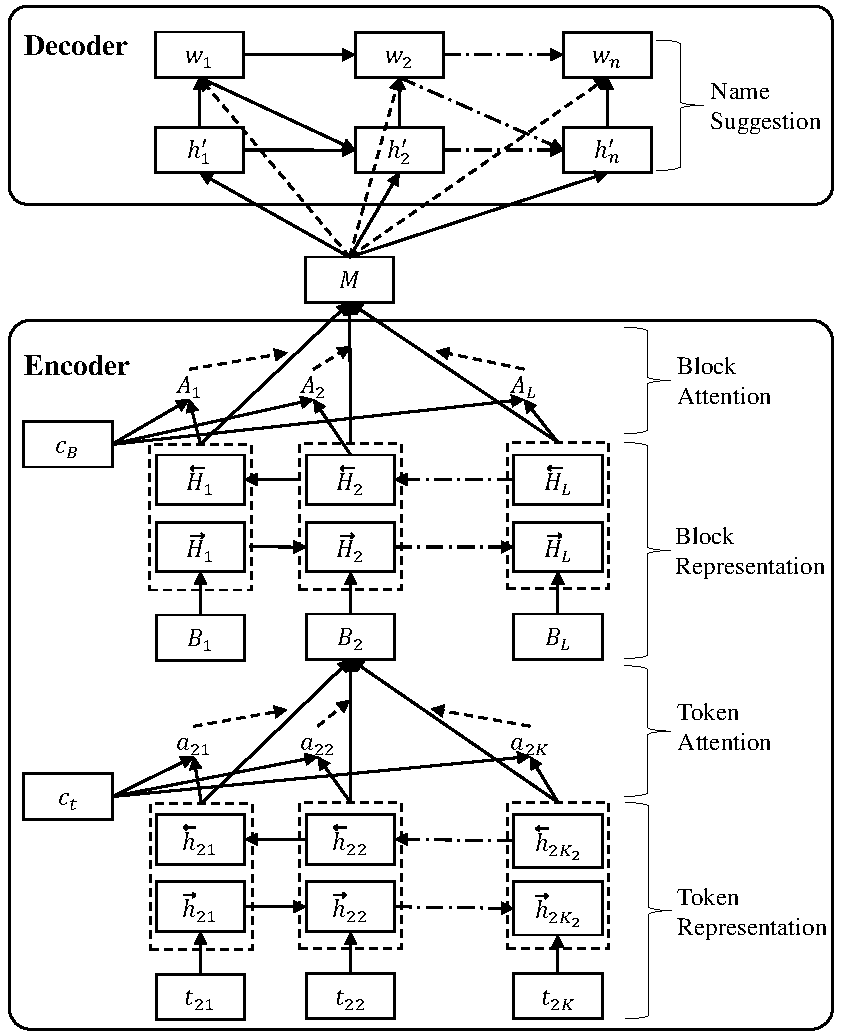
\includegraphics[width=0.65\textwidth]{architecture.pdf}
	\caption{Architecture of Method Name Suggestion.}
	\label{fig:arch}
\end{figure}

如图~\ref{fig:arch}所示,编码器对代码片段的表示分为两个阶段:在第一阶段,给定输入的词项序列,学习基
本代码块的表示;在第二阶段,以基本代码块序列列作为输入,学习整个代码片段(函数体)的表示。 在解码阶
段,以代码片段的表示作为输入,使用门控循环单元~\cite{Kyunghyun2014Learning}模型学习组成函数名的词项
序列在代码片段上的条件分布。同样,在计算当前隐藏状态$h_t'$时考虑上一个时刻的输出$w_{t-1}$,使模型能
快速收敛。

基于层次注意力网络的函数名推荐模型,其输入是由代码基本块序列构成的代码片段,输出是由词项序列构成的函
数名。给定函数$m$,将其表示为由代码基本块组成的序列$m=(B_1,B_2, \dots, B_L)$,每个基本块由词项序列表
示,例如$B_2 = (t_{21}, \dots, t_{2K_2})$,其中$K_2$为代码基本块$B_2$中所包含的词项的个数。模型的输
出为词项序列$(w_1, \dots, w_n)$,表示预测的函数名。需要注意的是,输入和输出序列的长度可以不一致,事
实上,与代码的长度相比,函数名的长度通常非常短,因此为给定代码片段预测函数名的困难较大。

编码器首先根据输入的代码基本块序列,通过层次注意力网络将函数体表示为一个固定长度的向量$M$:
\begin{equation}
M = f({B_1, \dots, B_L}) \,.
\label{eq:encoder}
\end{equation}
然后解码器依次预测组成函数名的词项,根据上一个时刻的词项和解码器的输出向量$M$,预测当前时刻的词项:
\begin{equation}
P(w_j|\{w_1, \dots, w_{j-1}\}, M) = g(\{w_1, \dots, w_{j}\}, M) \,,
\label{eq:decoder}
\end{equation}
其中$g$的输出为一个概率,表示根据代码片段的表示向量$M$和上一个时刻的输出词项$w_{j-1}$,预测当前词项
为$w_j$的概率,本文使用softmax激活函数使函数$g$的输出为一个概率值。

将解码器和编码器联合起来,能够学习关于函数名的词项序列$w$在由词项组成的代码段$t$上的条件分布
$p(y|t)$,最后通过最大条件对数似然来优化该联合模型:
\begin{equation}
\max \limits_{\bm\theta} \frac{1}{N}\sum_{n=1}^{N} \log p_{\bm\theta}(\bm w_n | 
\bm t_n) \,,
\label{eq:loss}
\end{equation}
其中$N$表示训练样本的个数,$\bm\theta$为模型中的参数,通过使用随机梯度下降来优化模型的参数。

\subsection{代码段表示}
为了提高模型的抽象和总结能力,本文将函数体拆分为多个代码基本块,每个代码块作为执行函数子功能的最小单
元,通过注意力机制学习不同代码基本块对函数名预测的重要性。

\begin{Definition}
    代码基本块。代码基本块为顺序执行的代码语句,每个代码块有且只有一个入口和一个出口。
\end{Definition}

给定函数体$m$,通过算法~\ref{alg:block}将其表示为由代码基本块组成的序列,即$m=(B_1,B_2, \dots,
B_L)$。其中控制语句集合$V$为包括条件语句(例如循环、分支的条件语句)、\textit{break}语句、
\textit{contibue}语句、返回语句、异常语句和结束语句。

\begin{algorithm}[H]
\caption{代码基本块提取算法}\label{alg:block}
\KwIn{函数$m$,控制语句集合$V$;}\\
\KwOut{代码基本块序列$b$;}\\
获取函数$m$中的所有代码$S$;\\
将函数$m$的第一行代码$S_1$放入代码基本块$B_1$中;\\
初始化$i=1$;\\
初始化$j=2$;\\
\While {$j \leq |S|$} {
   \If {$S_j==\text{"\}"}$} {
        \textbf{contibue};\\
    }
    \If {$S_j$ in $V$} {
        //此时语句$S_j$为控制语句\\
        更新$i=i+1$;\\
    }
    将语句$S_j$追加至代码基本块$B_i$中;\\
}
\textbf{return} $b=(B_1,B_2,\dots,B_L)$。
\end{algorithm}

以图~\ref{stop}中的示例代码为例,
$m=\{(try,\{), (logger,info,...), (if,bin,Log,...), (logger,infor,...,null), (catch,(,Exception,e,),) ,(throw,new,Runtime,Exception,(,e,),)\}$。


\subsection{基于层次注意力网络的编码器}
\subsection{基于GRU的序列解码器}
\subsubsection{GRU}
\subsection{集束搜索}
\section{实验设置}
\subsection{数据集和对比实验}
去掉出现过的Self替代

\subsection{评价指标}
\section{实验结果}
\section{讨论}
\section{本章小结}
